\documentclass{article}
\usepackage[utf8]{inputenc}
\usepackage[margin=0.70in]{geometry}
\usepackage{graphicx} %插入图片的宏包
\usepackage{float} %设置图片浮动位置的宏包
\usepackage{subfigure} %插入多图时用子图显示的宏包

\title{HW2.2: Parallelizing a Particle Simulation}
\author{Andrew Chen, Brian Park, Xuan Jiang}
\date{March 2022}

\begin{document}

\maketitle
\section{Collaboration and Introduction}
Everyone on the team contributed equally. Everyone started off the exploration of MPI together. Xuan, Brian and Andrew was able to explore how MPI Send and Receive works. Andrew tried to divide columns of bins among each process while Brian and Xuan used a row approach. We ended up using Brian's approach. Brian was able to figure out how to add MPI directives to optimize code. Brian figured out how to solve the segmentation fault and finally put everything work. Everyone contributed equally to the report and everyone contributed to the group repository equally.

We used a variety of techniques to optimize the problem of parallelizing a particle simulation.
In the remainder of this report, we describe each of our optimizations in our final submission,
present results with evidence that they work, and describe attempted optimizations that did not
noticeably improve overall our performance.

\section{$O(N)$ time plots and description of data structures} 

\subsection{Data Structures}
Used the same binning idea that we derived from homework 2-1

To be more specific:
We defined our bins as vectors:

\verb|typedef vector<particle_t*> bin_t;|

\verb|bin_t* bins;|

We make sure that particles are stored in bins. The number of bins is fixed which is why we use an array of bins. The bins themselves
change in size each simulation as they move around, which is why we use \verb|std::vector|.
\subsection{log-log plots}
\begin{figure}[H] %H为当前位置,!htb为忽略美学标准,htbp为浮动图形
\centering %图片居中
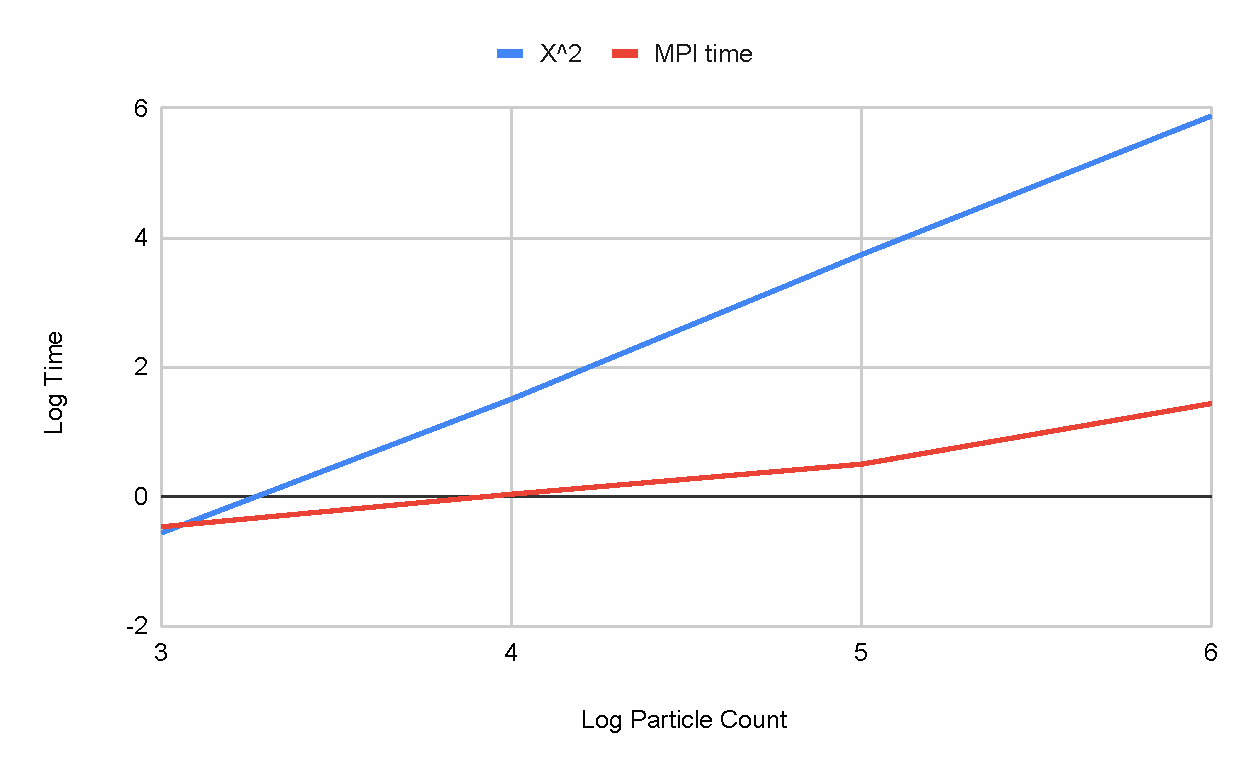
\includegraphics[width=0.7\textwidth]{loglog.pdf} %插入图片,[]中设置图片大小,{}中是图片文件名
\caption{log} %最终文档中希望显示的图片标题
\label{log} %用于文内引用的标签
\end{figure}

\section{MPI}


\subsection{Communication and Design Choice}
For MPI, it was much harder to implement due to explicit communication. We mainly took use of communication primitives such as \verb|MPI_Isend| and \verb|MPI_Irecv|. We only used this to explicitly send or receive neighboring particles when computing \verb|apply_force()|. Note that we only focused on moving between rows in a 1D layout. We found moving bins by a grid, in a 2D layout is much harder to implement. Given more time, we would've tackled the 2D layout. For rebinning, using \verb|MPI_Allgather| and \verb|MPI_Allgatherv|. We didn't want to deal with implementing additional data structure such as creating a ghost buffer or halo zone. Rather, we kept it simple and implemented All-to-All communication so that we can just rebin. We would need to synchronize before moving to the next step anyways, so this was the safest approach as well in order to achieve correctness. This is actually the same approach we took in OpenMP solution, but due to communication bottleneck in a distributed system, implementing explicit send and receive primitives may have been the more appropriate and tedious programming model. Due to the time it takes to debug and the performance we would achieve, we just stuck to this implementation. For \verb|gather_for_save()|, we implemented \verb|MPI_Gather| and \verb|MPI_Gatherv|. The reason why we used two gather version is because the sizes to collect are not uniform, so first we must calculate the size so that we can concatenate them properly in the second call to gather that uses the v version, indicating variable length buffer. This is a many to one collective communication and was necessary to communicate everything to the driver node to check for correctness when we save to output. The most difficult part of implementing gather was getting displacement right and how to collectively communicate data from different processes.

Some design choices we made were mainly simple, to ease debugging and development. Along with the grid partitioning, we also had to be mindful of how we think about programming a SPMD model. Becuase the exact same code is being run at the same time, we had to make sure we also synchronize and think åcreatively how to distribute computation across partitions of data. The use of \verb|rank| was useful, and we figured out a way to make this scalable with various number of nodes and processes that MPI and the KNL nodes can provide. We partitioned it such that each process or rank will be allocated a row of the grid space data structure. If we have less ranks than rows provided by the working set, we spill over and have ranks allocate more than one row for computation, denoted by \verb|leftover_processes|. Not proceeding with a rank to 2D mesh allocation may have affected performance, as load balancing could improve. With 2D, you could have more ranks do less computation, thus also potentially minimizing communication bottleneck between proceses.

\subsection{Can We Do Better?}

\section{Speed up plots and discussion}
\subsection{Weak Scaling}
\begin{figure}[H] %H为当前位置,!htb为忽略美学标准,htbp为浮动图形
\centering %图片居中
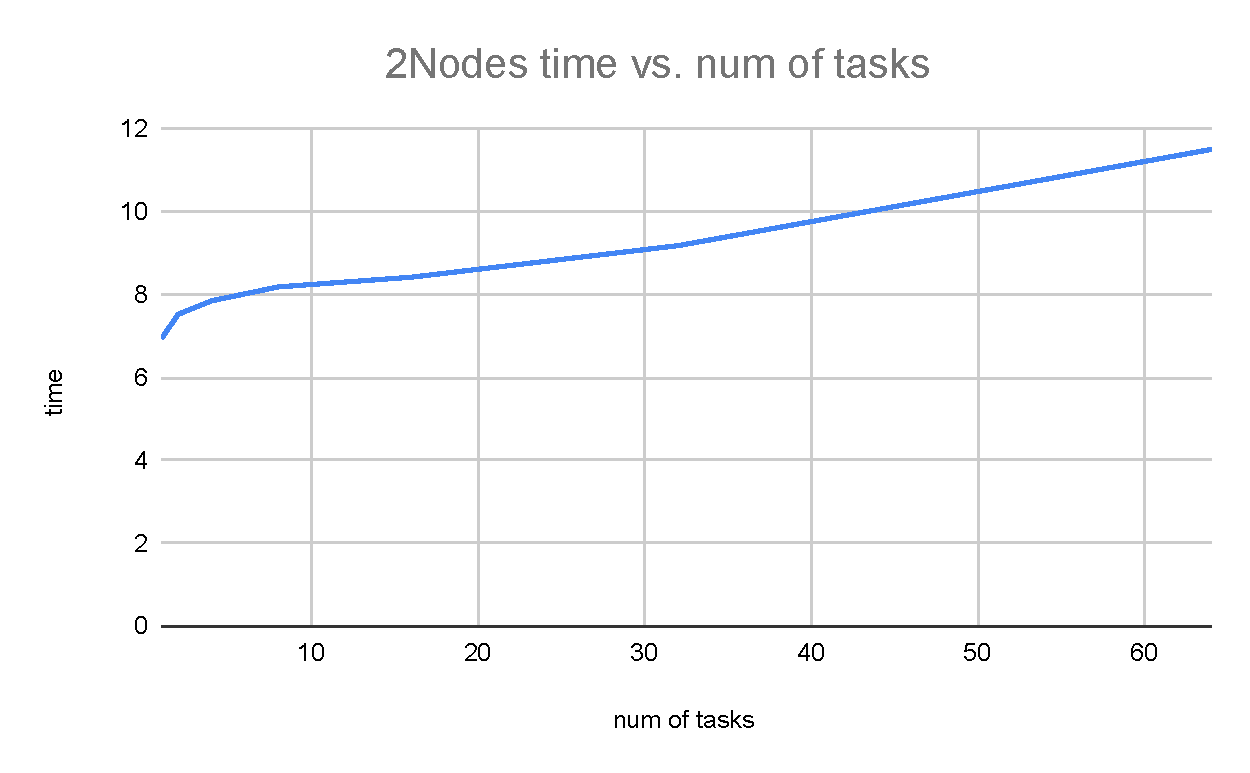
\includegraphics[width=0.7\textwidth]{2Nodes time vs. num of tasks.pdf} %插入图片,[]中设置图片大小,{}中是图片文件名
\caption{2Nodes time vs. num of tasks} %最终文档中希望显示的图片标题
\label{2Nodes time vs. num of tasks} %用于文内引用的标签
\end{figure}

We are only seeing a little jump on from 1 task to 2 tasks and then we are remaining good performance on increasing number of tasks by two times.


\begin{figure}[H] %H为当前位置,!htb为忽略美学标准,htbp为浮动图形
\centering %图片居中
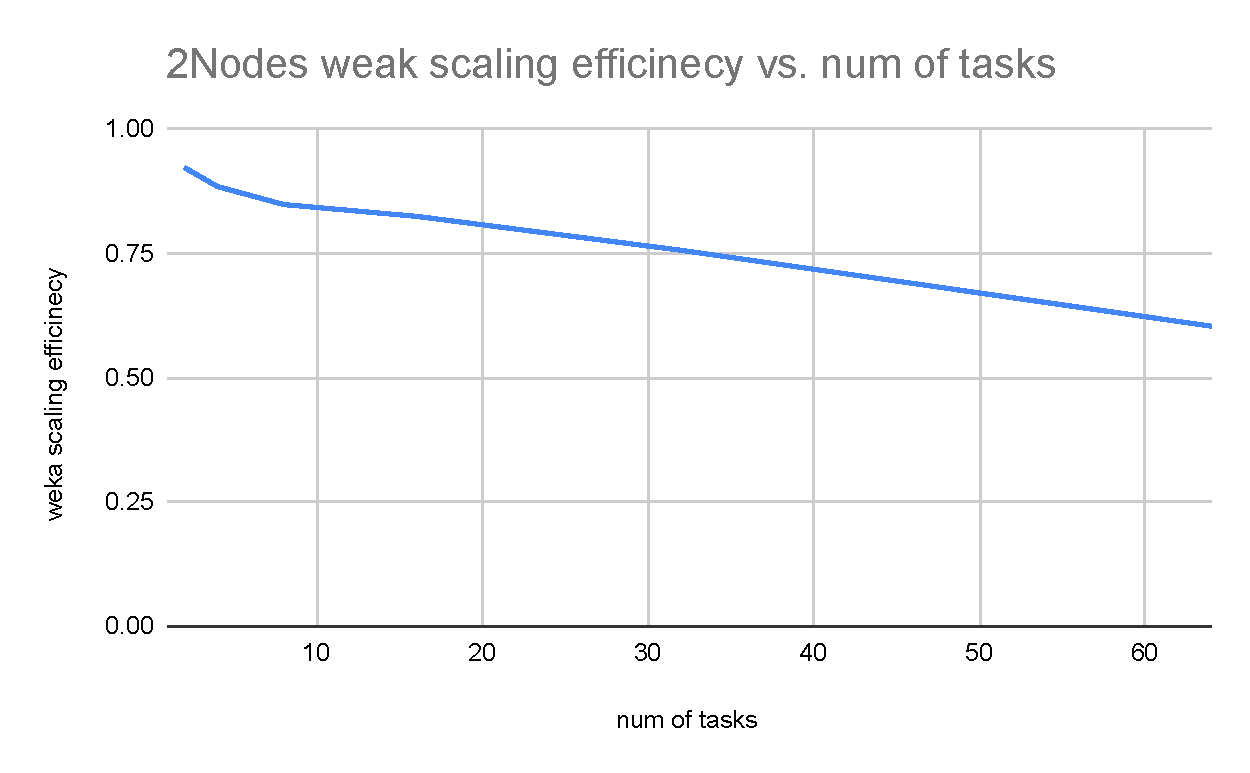
\includegraphics[width=0.7\textwidth]{2Nodes weak scaling efficinecy vs. num of tasks.pdf} %插入图片,[]中设置图片大小,{}中是图片文件名
\caption{2Nodes weak scaling efficiency vs. num of tasks} %最终文档中希望显示的图片标题
\label{2Nodes weak scaling efficinecy vs. num of tasks} %用于文内引用的标签
\end{figure}

We can see that our weak scaling efficiency is highest while we are using 2 processor which is 88.43\% and when we increasing the number of of processors and number of particles by the same times, the weak scaling efficiency is going all the way down to 60.34\%, but it's still pretty good.

\subsection{Strong Scaling}
We tested both for one node and two nodes. And finally, we test up to 2 nodes and 1,500,000 particles.

One Node:
\begin{figure}[H] %H为当前位置,!htb为忽略美学标准,htbp为浮动图形
\centering %图片居中
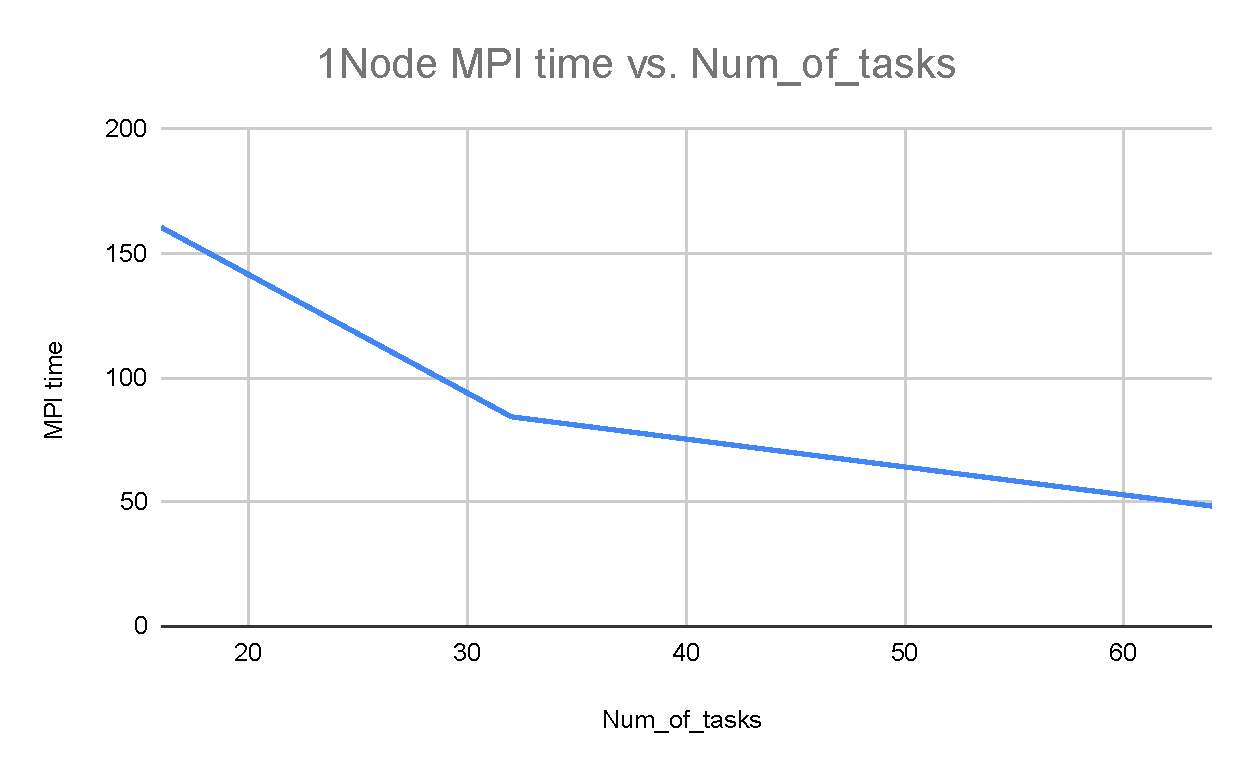
\includegraphics[width=0.7\textwidth]{1Node MPI time vs. Num_of_tasks.pdf} %插入图片,[]中设置图片大小,{}中是图片文件名
\caption{1Node MPI time vs. Num of tasks} %最终文档中希望显示的图片标题
\label{1Node MPI time vs. Num_of_tasks} %用于文内引用的标签
\end{figure}
We are only seeing a little jump on from 16 task to 32 processors and then we are remaining good performance on increasing number of processors by two times.

\begin{figure}[H] %H为当前位置,!htb为忽略美学标准,htbp为浮动图形
\centering %图片居中
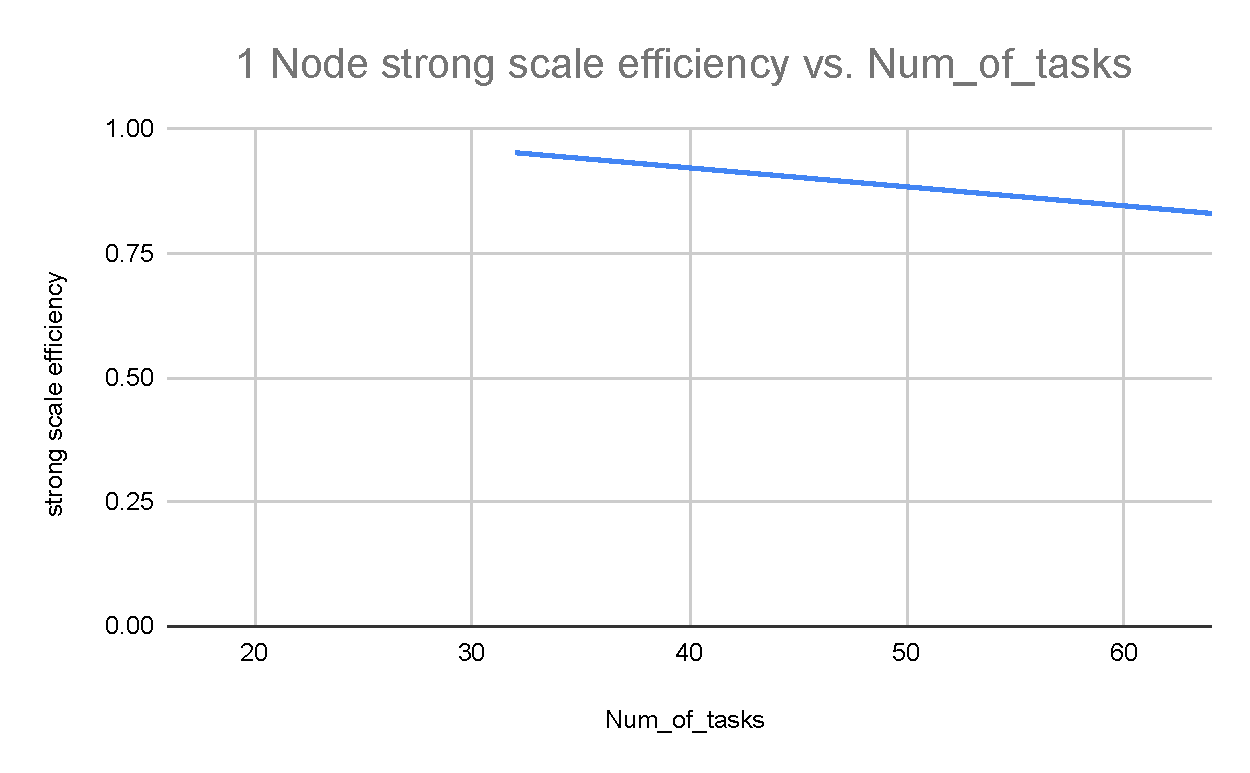
\includegraphics[width=0.7\textwidth]{1 Node strong scale efficiency vs. Num_of_tasks.pdf} %插入图片,[]中设置图片大小,{}中是图片文件名
\caption{1 Node strong scale efficiency vs. Num of tasks} %最终文档中希望显示的图片标题
\label{1 Node strong scale efficiency vs. Num_of_tasks} %用于文内引用的标签
\end{figure}

We can see that our weak scaling efficiency is highest while we are using 32 tasks which is 95.24\% and when we increasing the number of of tasks and number of particles by the same times, the weak scaling efficiency is going all the way down to 83.03\%, but it's still pretty good.

Two Nodes:
\begin{figure}[H] %H为当前位置,!htb为忽略美学标准,htbp为浮动图形
\centering %图片居中
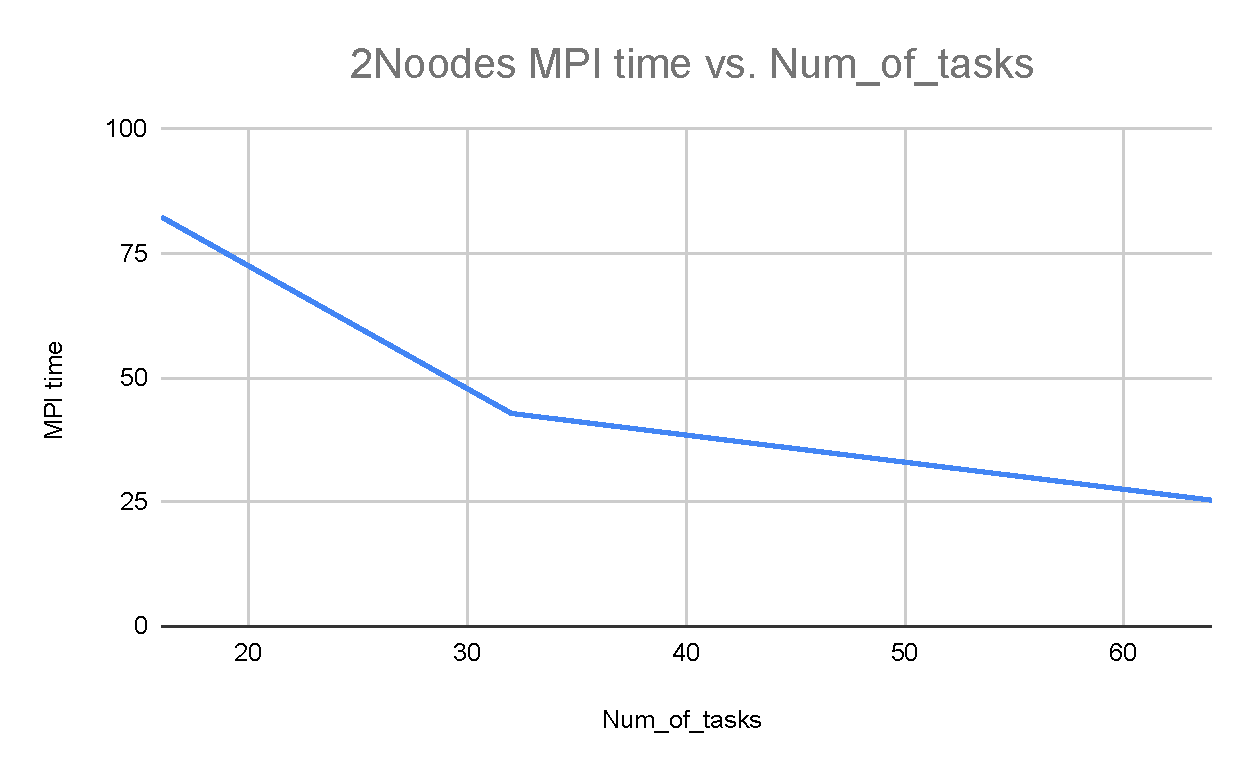
\includegraphics[width=0.7\textwidth]{2Nodes MPI time vs. Num_of_tasks.pdf} %插入图片,[]中设置图片大小,{}中是图片文件名
\caption{2 Node MPI time vs. Num of tasks} %最终文档中希望显示的图片标题
\label{2 Nodes MPI time vs. Num_of_tasks} %用于文内引用的标签
\end{figure}

Again, We are only seeing a little jump on from 16 task to 32 processors and then we are remaining good performance on increasing number of processors by two times.


\begin{figure}[H] %H为当前位置,!htb为忽略美学标准,htbp为浮动图形
\centering %图片居中
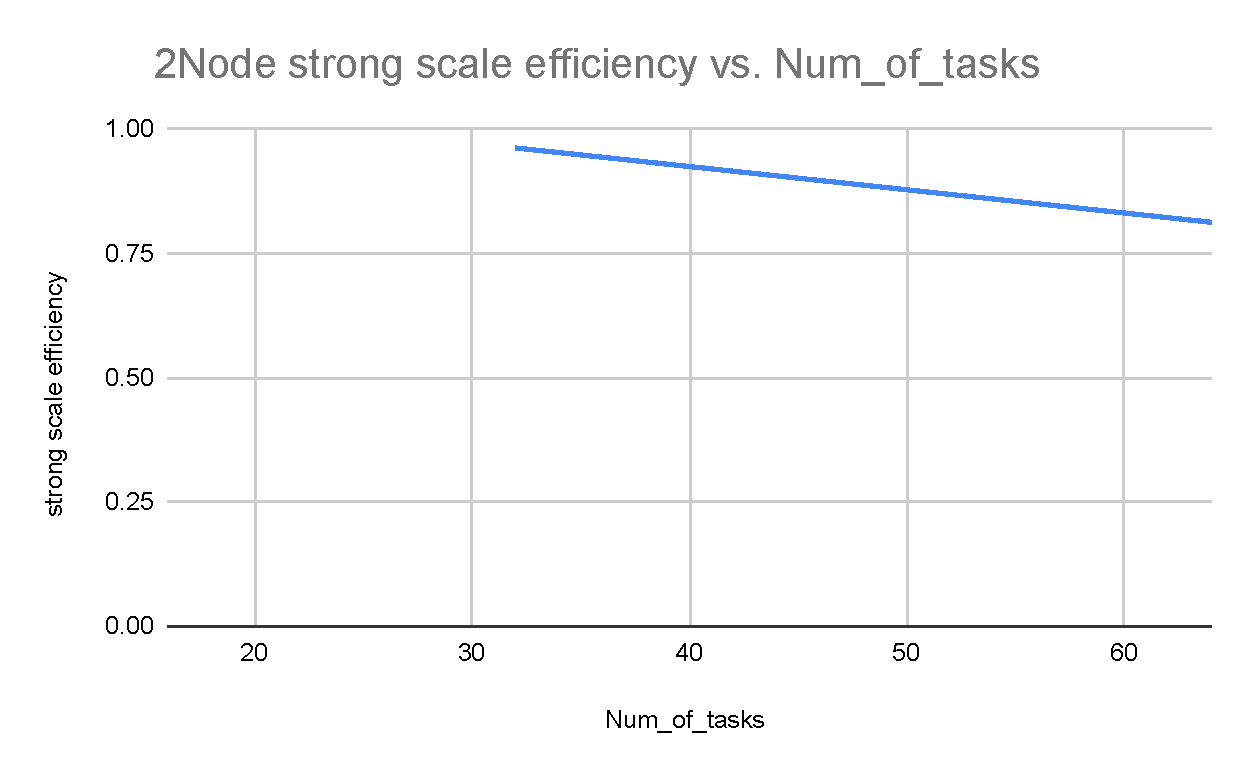
\includegraphics[width=0.7\textwidth]{2Node strong scale efficiency vs. Num_of_tasks.pdf} %插入图片,[]中设置图片大小,{}中是图片文件名
\caption{2Node strong scale efficiency vs. Num of tasks} %最终文档中希望显示的图片标题
\label{2Node strong scale efficiency vs. Num_of_tasks} %用于文内引用的标签
\end{figure}

We can see that our weak scaling efficiency is highest while we are using 32 tasks which is 96.20\% and when we increasing the number of of tasks and number of particles by the same times, the weak scaling efficiency is going all the way down to 81.24\%, but it's still pretty good.


\section{Performance Breakdown}
For this we have communication time, computation time and synchronization time. Our total time is 24.4984s for 1.5 million particles, and we spend most of our communication time on mpi finalize, however, message sending and receiving didn't take a lot. Both of them take nearly 2-3\% of the time. Interestingly, gather and all gather took 20-30\% of the time, indicating that communication of all processes definitely takes a significant hit on performance. And they scale almost linearly proportional with p. Since we are using non-blocking communication, we measure the time used on MPI_Wait.

For computation, we left the code without any explicit barriers, and for synchronization, we left barriers on. We see that they have nearly the same times. We used print statements as we didn't really know how to utilize the profiling tools, the learning curve for using it was very steep.


% Your write-up should contain:


% A plot in log-log scale that shows that your parallel codes performance and a description of the data structures that you used to achieve it.





% Speedup plots that show how closely your MPI code approaches the idealized p-times speedup and a discussion on whether it is possible to do better. Both strong and weak scaling. Test up to 2 nodes and 1,500,000 particles.

% Where does the time go? Consider breaking down the runtime into computation time, synchronization time and/or communication time. How do they scale with p?

% Notes:

% Your grade will mostly depend on three factors:

% Scaling sustained by your codes on the Cori supercomputer (varying n).

% Performance sustained by your codes on the Cori supercomputer.

% Explanations of your methodologies and the performance features you observed (including what didn't work).

\end{document}
For this we have communication time, computation time and synchronization time. Our total time is 24.4984s for 1.5 million particles, and we spend most of our communication time on mpi finalize, however, message sending and receiving didn't take a lot.